\chapter{コンフリクト — 変更の衝突を解決する}

\section{この章で学ぶこと}

チーム開発において、複数人が同時に作業を進めることはごく日常的な光景です。しかし、2人以上の開発者が同じファイルの同じ箇所をそれぞれ異なる形で変更してしまった場合、Gitはどちらの変更を採用すべきか判断できなくなります。この状態を\textbf{コンフリクト（conflict、競合）}と呼びます。

コンフリクトという言葉を聞くと、「怖い」「壊れたらどうしよう」と身構える初学者が少なくありません。しかし、コンフリクトはGitが「ここは人間の判断が必要です」と教えてくれているだけであり、正しく対処すれば何も失われることはありません。むしろ、コンフリクトを適切に解決できるスキルは、チーム開発において非常に重要な能力の一つです。

この章では、以下の内容を学びます。

\begin{itemize}
  \item コンフリクトとは何か、なぜ発生するのかを具体例で理解する
  \item コンフリクトが発生する4つの典型的な場面を知る
  \item コンフリクトマーカーの読み方を1行ずつ丁寧に学ぶ
  \item 手動・VS Code・コマンドの3通りの解決方法を習得する
  \item マージやリベースの中止方法を知る
  \item コンフリクトを未然に防ぐチーム運営のプラクティスを身につける
\end{itemize}

\section{コンフリクトとは何か}

\subsection{日常のたとえで理解する}

コンフリクトを日常生活に例えてみましょう。あなたとチームメンバーの田中さんが、同じ共有ドキュメントを編集しているとします。あなたは「会議の日程は火曜日」と書き換え、同じ時間帯に田中さんは「会議の日程は木曜日」と書き換えました。このとき、最終的な正解は「火曜日」なのか「木曜日」なのか、コンピュータには判断のしようがありません。これがコンフリクトです。

\subsection{Gitにおけるコンフリクトの仕組み}

Gitは非常に賢いマージアルゴリズムを持っており、ほとんどの場合は自動的に変更を統合してくれます。たとえば、あなたが \cmd{README.md} の1行目を変更し、田中さんが同じファイルの50行目を変更した場合、Gitは「別々の箇所の変更だから両方取り込めばよい」と判断して自動マージを行います。

しかし、\textbf{同じファイルの同じ行（または非常に近い行）を異なる内容に変更した場合}、Gitは自動マージを諦め、人間に判断を委ねます。これがコンフリクトの正体です。

\begin{lstlisting}[language={}]
main:     "Hello World"  →  "Hello GitHub"    ← mainブランチで変更
                \
feature:         →  "Hello Git"               ← featureブランチでも同じ箇所を変更

→ どちらを採用すべきかGitには判断できない = コンフリクト発生
\end{lstlisting}

この図の例では、元々 \cmd{"Hello World"} だった文字列を、mainブランチでは \cmd{"Hello GitHub"} に変更し、featureブランチでは \cmd{"Hello Git"} に変更しています。Gitにとって、どちらが「正しい」変更なのかを知る手がかりはありません。そのため、開発者自身に「どうしますか？」と問いかけるわけです。

\subsection{コンフリクトは「エラー」ではない}

ここで強調しておきたいのは、コンフリクトはエラーやバグではないということです。コンフリクトは、チーム開発における正常な出来事です。Gitが「私には判断できないので、あなたが決めてください」と言っているだけであり、リポジトリが壊れたわけでも、データが失われたわけでもありません。落ち着いて解決すれば、何の問題もないのです。

\section{コンフリクトが発生する場面}

コンフリクトは、2つの異なる変更履歴を統合しようとするあらゆる場面で発生する可能性があります。具体的には、以下の4つの操作が代表的です。

\subsection{git merge でブランチを統合するとき}

最も一般的なコンフリクトの発生場面です。featureブランチでの作業が完了し、mainブランチにマージしようとしたとき、mainブランチ側でも同じ箇所が変更されていると、コンフリクトが発生します。

\begin{lstlisting}[language=bash]
git switch main
git merge feature/login
# Auto-merging src/app.py
# CONFLICT (content): Merge conflict in src/app.py
# Automatic merge failed; fix conflicts and then commit the result.
\end{lstlisting}

このメッセージを見たら、慌てる必要はありません。Gitは「\cmd{src/app.py} で自動マージを試みたが、コンフリクトが発生した。コンフリクトを解決してからコミットしてください」と親切に教えてくれています。

\subsection{git pull でリモートの変更を取り込むとき}

チームメンバーがリモートリポジトリにpushした変更と、あなたがローカルで行った変更が同じ箇所に及んでいる場合、\cmd{git pull} を実行した際にコンフリクトが発生します。これは本質的には \cmd{git merge} と同じ現象です（\cmd{git pull} は内部的に \cmd{git fetch} + \cmd{git merge} を行っているため）。

\subsection{git rebase でブランチの基点を付け替えるとき}

リベース操作では、あなたのコミットを1つずつ新しい基点の上に適用し直します。この過程で、いずれかのコミットが基点側の変更と衝突した場合、コンフリクトが発生します。リベースの場合、複数のコミットを順番に適用するため、1回のリベースで複数回コンフリクトが発生する可能性がある点に注意が必要です。

\subsection{git cherry-pick で特定のコミットを取り込むとき}

別のブランチから特定のコミットだけを取り込む \cmd{git cherry-pick} でも、取り込もうとするコミットが現在のブランチの内容と衝突すれば、コンフリクトが発生します。

\subsection{コンフリクト発生時のgit status}

コンフリクトが発生したら、まず \cmd{git status} で状況を確認しましょう。

\begin{lstlisting}[language=bash]
git status
# On branch main
# You have unmerged paths.
#   (fix conflicts and run "git commit")
#
# Unmerged paths:
#   (use "git add <file>..." to mark resolution)
#       both modified:   src/app.py
\end{lstlisting}

\cmd{both modified}（両方で変更されている）という表示が、コンフリクトが起きているファイルを示しています。複数のファイルでコンフリクトが発生している場合は、ここに複数のファイルが列挙されます。

\section{コンフリクトマーカーの読み方}

コンフリクトが発生すると、Gitは該当ファイルの中に\textbf{コンフリクトマーカー}と呼ばれる特別な記号を挿入します。このマーカーは、「ここから先が衝突している部分ですよ」と示す目印です。初めて見ると少し面食らうかもしれませんが、構造はシンプルです。

\subsection{マーカーの全体像}

\begin{lstlisting}[language=python]
def greet():
<<<<<<< HEAD
    return "Hello GitHub"
=======
    return "Hello Git"
>>>>>>> feature/login
\end{lstlisting}

このコードを1行ずつ読み解いていきましょう。

\subsection{各行の意味}

\textbf{\cmd{<<<<<<< HEAD}}（7つの \cmd{<} と「HEAD」）

この行は「ここからが、あなたが今いるブランチ（マージ先、つまりHEAD）の変更内容ですよ」という開始マーカーです。HEADとは、現在チェックアウトしているブランチの最新コミットを指すGitの用語です。マージ操作の場合、これは「マージ先」のブランチ、つまりあなたが \cmd{git merge} を実行したときにいたブランチの内容です。

\textbf{\cmd{    return "Hello GitHub"}}

これがHEAD側（マージ先ブランチ）の実際のコード内容です。この例では、mainブランチ上でgreet関数が \cmd{"Hello GitHub"} を返すように変更されていたことがわかります。

\textbf{\cmd{=======}}（7つの \cmd{=}）

この行は区切り線です。ここを境にして、上がマージ先の変更、下がマージ元の変更となります。いわば、2つの変更を隔てる「仕切り」の役割を果たしています。

\textbf{\cmd{    return "Hello Git"}}

これがマージ元ブランチの実際のコード内容です。featureブランチでは、greet関数が \cmd{"Hello Git"} を返すように変更されていたことがわかります。

\textbf{\cmd{>>>>>>> feature/login}}（7つの \cmd{>} とブランチ名）

この行は「ここまでがマージ元ブランチ（feature/login）の変更内容ですよ」という終了マーカーです。ブランチ名が表示されるので、どのブランチの変更なのかを識別できます。

\subsection{マーカーの構造を表にまとめると}

\begin{table}[htbp]
\centering
\begin{tabular}{llp{6cm}}
\hline
\textbf{マーカー} & \textbf{意味} & \textbf{覚え方} \\
\hline
\cmd{<<<<<<< HEAD} & マージ先（現在のブランチ）の変更の開始 & \cmd{<} は「こちら側」を指す矢印 \\
\cmd{=======} & 2つの変更の区切り線 & 「ここから先は相手側」 \\
\cmd{>>>>>>> branch-name} & マージ元ブランチの変更の終了 & \cmd{>} は「あちら側」を指す矢印 \\
\hline
\end{tabular}
\end{table}

このマーカーの読み方を理解しておけば、どんなに長いファイルでコンフリクトが発生しても、落ち着いて対処できます。なお、1つのファイル内に複数のコンフリクト箇所がある場合、マーカーのセットが複数回登場します。すべてのマーカーを解決しなければ、コンフリクトの解決は完了しません。

\begin{figure}[htbp]
\centering
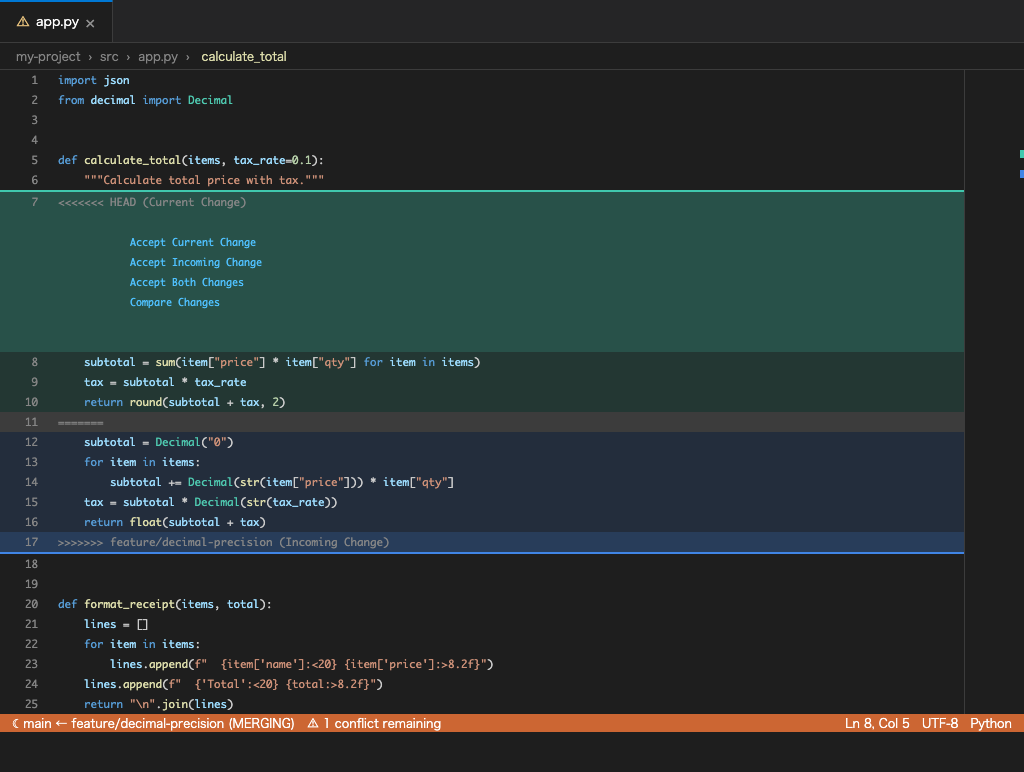
\includegraphics[width=0.95\textwidth]{images/vscode-conflict.png}
\caption{テキストエディタで表示されたコンフリクトマーカーの例}
\end{figure}

\section{手動で解決する方法}

コンフリクトの解決は、突き詰めれば「コンフリクトマーカーを取り除いて、最終的にあるべきコードにする」という作業です。テキストエディタでファイルを開き、自分の判断でコードを編集します。解決のパターンは大きく3つあります。

\subsection{パターン1：片方の変更を採用する}

最もシンプルなパターンです。2つの変更のうち、どちらか一方が正しいと判断できる場合、一方を残してもう一方とすべてのマーカーを削除します。

たとえば、mainブランチの変更（\cmd{"Hello GitHub"}）を採用する場合、コンフリクト箇所を以下のように書き換えます。

\begin{lstlisting}[language=python]
def greet():
    return "Hello GitHub"
\end{lstlisting}

マーカー行（\cmd{<<<<<<<}、\cmd{=======}、\cmd{>>>>>>>}）はすべて削除し、採用する側のコードだけを残す点がポイントです。マーカーが1つでも残っていると、プログラムとして正しく動作しません。

\subsection{パターン2：両方の変更を統合する}

2つの変更がどちらも必要な場合、両方の意図を活かした新しいコードを書きます。

\begin{lstlisting}[language=python]
def greet():
    return "Hello GitHub and Git"
\end{lstlisting}

この例では、「GitHub」と「Git」のどちらも盛り込む形で統合しています。両方の変更者の意図を尊重しつつ、整合性のあるコードにすることが求められます。

\subsection{パターン3：完全に書き直す}

どちらの変更もそのままでは不十分だと判断した場合、コンフリクト箇所をまったく新しいコードに書き直すことも可能です。

\begin{lstlisting}[language=python]
def greet(target="World"):
    return f"Hello {target}"
\end{lstlisting}

この例では、固定文字列を返すのではなく引数で切り替えられる設計に変更しています。コンフリクトをきっかけに、より良い実装に改善することは、実際のチーム開発でもよくあることです。

\subsection{解決後の操作：add と commit}

どのパターンで解決したとしても、最終的な手順は共通です。

\begin{lstlisting}[language=bash]
# 1. 解決したファイルをステージに追加する
git add src/app.py

# 2. マージコミットを作成する
git commit -m "Merge feature/login: resolve greeting conflict"
\end{lstlisting}

\cmd{git add} は、「このファイルのコンフリクトは解決しました」とGitに伝える役割も担っています。コンフリクトが残ったままのファイルを \cmd{git add} しようとしても、マーカーが残っている限り問題の根本は解決していませんので、必ずマーカーをすべて削除してからaddしてください。

複数のファイルでコンフリクトが発生している場合は、すべてのファイルを解決してから一括でコミットします。

\begin{lstlisting}[language=bash]
git add src/app.py src/utils.py src/config.py
git commit -m "Merge feature/login: resolve all conflicts"
\end{lstlisting}

\section{VS Codeで解決する方法}

コンフリクトマーカーを手動で編集するのは確実な方法ですが、Visual Studio Code（VS Code）を使えば、より視覚的にわかりやすく、効率的にコンフリクトを解決できます。VS Codeは現在、最も広く使われているコードエディタの一つであり、Gitのコンフリクト解決機能が標準で組み込まれています。

\subsection{コンフリクト箇所の表示}

VS Codeでコンフリクトが発生しているファイルを開くと、コンフリクトマーカーの部分が色分けして表示されます。通常、HEAD側（現在のブランチ）の変更は緑色の背景で、マージ元の変更は青色の背景でハイライトされます。

\begin{figure}[htbp]
\centering
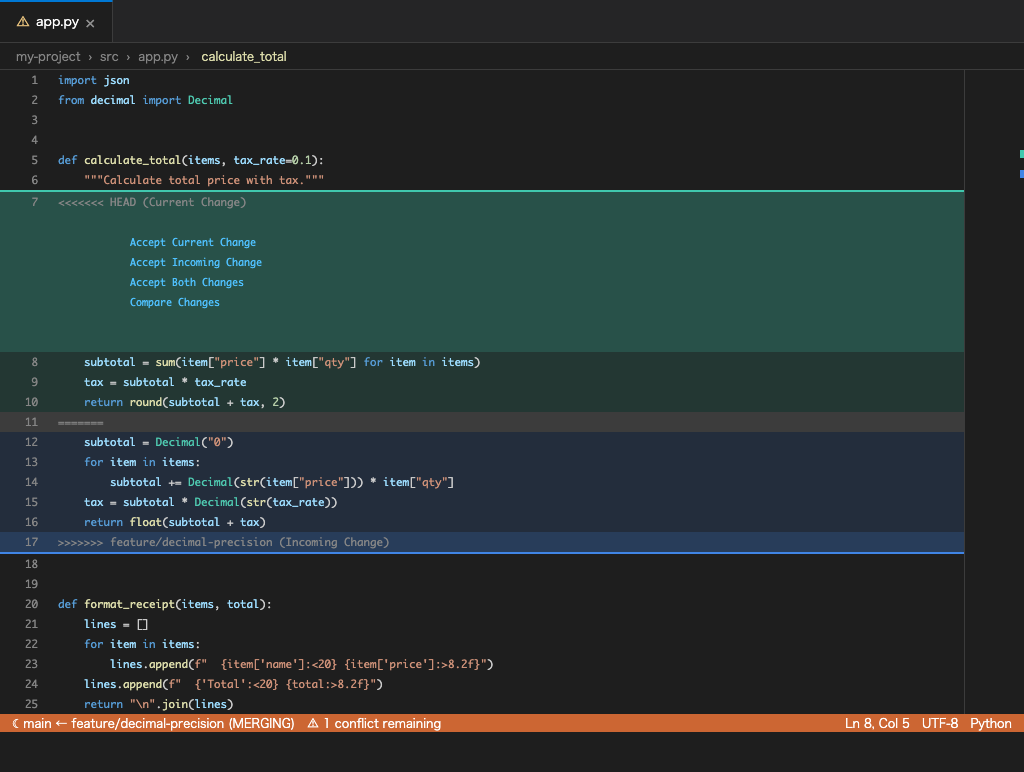
\includegraphics[width=0.95\textwidth]{images/vscode-conflict.png}
\caption{VS Codeのコンフリクト解決UI（色分けされたコンフリクト箇所とボタン）}
\end{figure}

\subsection{ワンクリック解決ボタン}

コンフリクト箇所の上部には、以下の4つのボタン（リンク）が表示されます。

\textbf{Accept Current Change（現在の変更を採用）}

HEAD側、つまりあなたが今いるブランチの変更を採用します。マージ元の変更は破棄されます。「自分の変更が正しい」と確信できる場合に使います。

\textbf{Accept Incoming Change（入ってくる変更を採用）}

マージ元ブランチの変更を採用します。HEAD側の変更は破棄されます。「相手の変更が正しい」「相手の変更のほうが新しい」という場合に使います。

\textbf{Accept Both Changes（両方の変更を採用）}

両方の変更を上下に並べてそのまま残します。ただし、この操作は機械的に2つのコードブロックを連結するだけなので、結果として文法的に正しくないコードになることもあります。必要に応じて、ボタンを押した後に手動で微調整してください。

\textbf{Compare Changes（変更を比較）}

2つの変更を横に並べて比較表示します。どちらを採用するか判断に迷うとき、差分を見比べるために使います。

\subsection{VS Codeのマージエディタ}

VS Code 1.70以降では、より高度な「3-way マージエディタ」も搭載されています。これは、左側にHEAD側の変更、右側にマージ元の変更、下部に最終結果を表示する3ペイン構成のエディタです。複雑なコンフリクトを解決する際に特に便利です。

コンフリクト解決後は、ターミナルに戻って通常どおり \cmd{git add} と \cmd{git commit} を実行します。

\section{コマンドで一括解決する方法}

ファイル数が多い場合や、「すべてのコンフリクトで一方の変更を採用する」と明確に決められる場合は、コマンドで一括解決するのが効率的です。Gitには \cmd{--ours} と \cmd{--theirs} というオプションが用意されています。

\subsection{--ours：自分の変更をすべて採用}

\begin{lstlisting}[language=bash]
git checkout --ours .
git add .
\end{lstlisting}

\cmd{--ours} は「自分（マージ先、HEAD側）の変更を採用する」という意味です。ピリオド（\cmd{.}）はカレントディレクトリ以下のすべてのファイルを対象にすることを示します。この操作により、コンフリクトが発生しているすべてのファイルで、HEAD側の内容が採用されます。

\subsection{--theirs：相手の変更をすべて採用}

\begin{lstlisting}[language=bash]
git checkout --theirs .
git add .
\end{lstlisting}

\cmd{--theirs} は「相手（マージ元ブランチ側）の変更を採用する」という意味です。たとえば、mainブランチの最新状態にfeatureブランチを合わせたい場合などに使います。

\subsection{注意点}

\cmd{--ours} と \cmd{--theirs} は非常に便利ですが、すべてのコンフリクト箇所で一律に片方を採用してしまうため、意図しない変更の喪失が起こりうる点に注意が必要です。「このコンフリクトはours、このコンフリクトはtheirs」と個別に判断したい場合は、ファイル単位で指定するか、手動で解決してください。

\begin{lstlisting}[language=bash]
# 特定のファイルだけ相手の変更を採用する
git checkout --theirs src/config.py
git add src/config.py
\end{lstlisting}

また、\cmd{--ours} と \cmd{--theirs} の意味はリベース中に逆転する点にも注意が必要です。リベースでは、まずHEADがリベース先のブランチに移動し、その上にあなたのコミットを1つずつ適用する仕組みのため、\cmd{--ours} がリベース先（相手側）、\cmd{--theirs} があなたのコミット（自分側）になります。混乱しやすいポイントなので覚えておきましょう。

\section{マージやリベースの中止方法}

コンフリクトが複雑で手に負えない場合、あるいは「そもそもこのマージをやるべきではなかった」と気づいた場合、操作を中止して元の状態に戻すことができます。中止しても何かが壊れることはありませんので、安心して使ってください。

\subsection{マージの中止}

\begin{lstlisting}[language=bash]
git merge --abort
\end{lstlisting}

\cmd{git merge --abort} は、マージ操作を中止し、マージを開始する前の状態に完全に戻します。コンフリクトマーカーが挿入されたファイルも元に戻ります。「やっぱりやめよう」と思ったら、迷わずこのコマンドを実行してください。

\subsection{リベースの中止}

\begin{lstlisting}[language=bash]
git rebase --abort
\end{lstlisting}

リベース中にコンフリクトが発生した場合も同様に、\cmd{git rebase --abort} で中止できます。リベースでは複数のコミットを順番に適用するため、途中でコンフリクトが何度も発生することがあります。「これは想定以上に複雑だ」と感じたら、一旦中止して戦略を練り直すのも賢い判断です。

\subsection{cherry-pickの中止}

\begin{lstlisting}[language=bash]
git cherry-pick --abort
\end{lstlisting}

\cmd{git cherry-pick} 中にコンフリクトが発生した場合も、\cmd{--abort} で中止できます。

\subsection{中止した後にやるべきこと}

操作を中止した後は、なぜコンフリクトが発生したのかを振り返りましょう。チームメンバーと会話して、作業の分担を見直したり、先にmainブランチの最新を取り込んでからマージし直したりすると、スムーズに解決できることが多いです。

\section{コンフリクトを予防するプラクティス}

コンフリクトは完全に防ぐことはできませんが、発生頻度を大幅に減らし、発生したとしても小規模に抑えるための工夫があります。以下のプラクティスをチームで実践すると、日々の開発がぐっとスムーズになります。

\subsection{こまめに pull / rebase する}

長期間mainブランチの変更を取り込まずに作業を続けると、mainとの差分がどんどん大きくなり、いざマージしようとしたときに大量のコンフリクトが発生しがちです。毎日の作業開始時に、mainの最新を取り込む習慣をつけましょう。

\begin{lstlisting}[language=bash]
# 毎朝の習慣にしたいコマンド
git switch main
git pull
git switch feature/my-work
git rebase main
\end{lstlisting}

この4行を日課にすることで、mainブランチとの乖離を最小限に抑え、コンフリクトが発生しても小さなうちに対処できます。

\subsection{小さなプルリクエストを心がける}

変更行数が多ければ多いほど、他の開発者の変更と衝突する確率は高まります。1つのプルリクエストは可能な限り小さく保ちましょう。目安として、変更が200〜300行を超えるようであれば、機能を分割して複数のプルリクエストに分けることを検討してください。小さなプルリクエストはレビューもしやすく、マージまでの時間も短くなるため、コンフリクトの発生リスクが下がります。

\subsection{担当ファイルを分ける}

チームメンバーが同時に同じファイルを編集する機会が多いほど、コンフリクトは発生しやすくなります。作業開始前にチームで簡単に共有し、「このファイルは今日は○○さんが触る」といった暗黙の了解を作ることで、衝突を減らせます。

もちろん、コードの構造自体を工夫して、1つの巨大なファイルに機能を詰め込むのではなく、適切にファイルを分割しておくことも重要です。

\subsection{rerere を有効にする}

\cmd{rerere}（reuse recorded resolution）は、Gitの隠れた便利機能の一つです。一度解決したコンフリクトのパターンをGitが記憶し、同じパターンのコンフリクトが再度発生した際に自動的に同じ解決を適用してくれます。

\begin{lstlisting}[language=bash]
# rerereを有効化（一度設定すればOK）
git config --global rerere.enabled true
\end{lstlisting}

たとえば、リベースを繰り返す運用をしているチームでは、同じコンフリクトが何度も発生することがあります。rerereを有効にしておけば、2回目以降は自動的に解決されるため、作業の手間が大幅に減ります。

rerereの名前は「re-use recorded resolution」の略で、文字どおり「記録した解決を再利用する」という機能です。地味ですが、長期的に見ると非常に大きな効果があります。

\subsection{チーム内でコミュニケーションをとる}

技術的な対策も重要ですが、最も効果的なのはチーム内のコミュニケーションです。「今からこのファイルを大きく変更する」「このモジュールのリファクタリングを始める」といった情報を事前に共有することで、意図しない衝突を避けることができます。SlackやTeamsなどのチャットツール、デイリースタンドアップミーティングなどを活用しましょう。

\section{まとめ}

この章では、Gitにおけるコンフリクト（変更の衝突）について、発生の仕組みから解決方法、予防策までを学びました。

コンフリクトは、同じファイルの同じ箇所を複数の開発者が異なる形で変更した際に発生します。Gitはコンフリクトマーカー（\cmd{<<<<<<<}、\cmd{=======}、\cmd{>>>>>>>}）を使って衝突箇所を示してくれるので、このマーカーの読み方を覚えておけば、どんなコンフリクトにも対処できます。

解決方法としては、テキストエディタでの手動解決、VS Codeの視覚的なGUI、\cmd{--ours} / \cmd{--theirs} を使ったコマンドでの一括解決の3通りがあります。状況に応じて使い分けてください。また、コンフリクトが手に負えない場合は \cmd{--abort} で安全に中止できることも覚えておきましょう。

そして何より、こまめなpull、小さなプルリクエスト、担当の分担、rerereの活用、チーム内のコミュニケーションといったプラクティスを日常的に実践することで、コンフリクトの発生頻度と深刻度を大幅に抑えることができます。

コンフリクトは怖いものではなく、チーム開発における自然な現象です。この章で学んだ知識があれば、自信を持って対処できるはずです。

次の章では、Gitの履歴操作コマンドを学びます。間違えてしまったコミットを取り消す方法、作業を一時退避する方法、消えてしまったコミットを救出する方法など、「過去を自在にたどる」テクニックを身につけましょう。
